
%(BEGIN_QUESTION)
% Copyright 2015, Tony R. Kuphaldt, released under the Creative Commons Attribution License (v 1.0)
% This means you may do almost anything with this work of mine, so long as you give me proper credit

Examine this schematic diagram sampled from Victor H. Todd's 1922 book {\it Protective Relays} showing a {\it reverse power} protection circuit for a DC power system whereby a generator typically supplies a load with power and maintains a storage battery in a continual state of full charge:

$$\epsfxsize=6in 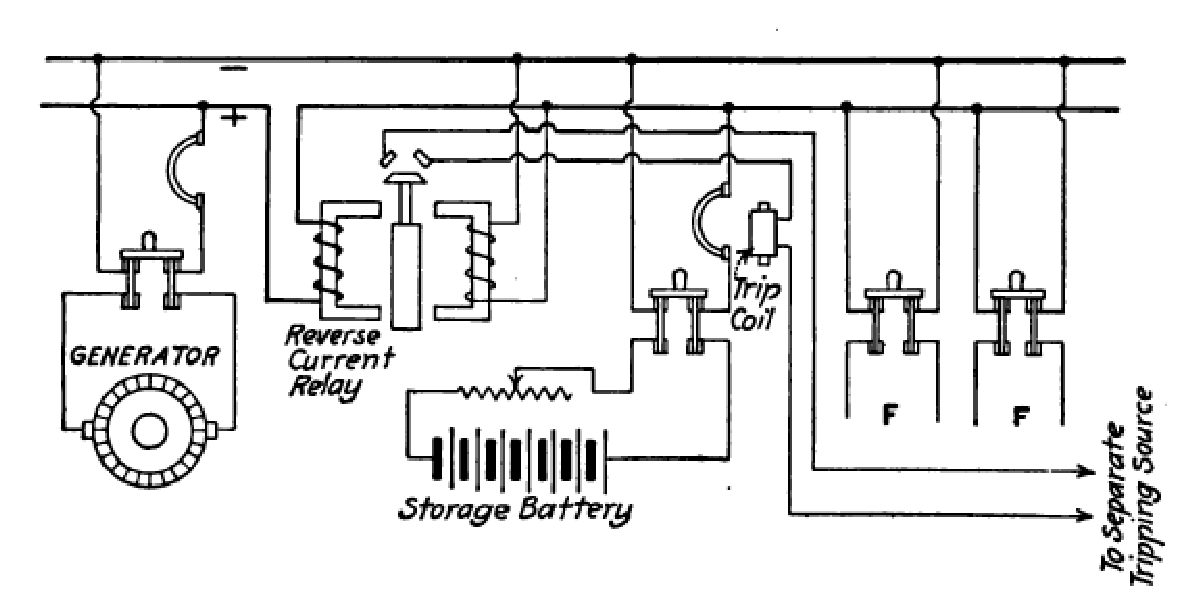
\includegraphics[width=15.5cm]{i02863x01.eps}$$

If the generator's mechanical prime mover ever fails (e.g. water gets shut off to the hydro turbine, engine runs out of fuel, etc.), the purpose of the directional relay is to trip the storage battery's breaker so that the storage battery does not discharge itself powering the generator as an electric motor.

\vskip 10pt

Examine this relay closely and determine how it fulfills its directional function.

\vskip 10pt

\underbar{file i02863}
%(END_QUESTION)





%(BEGIN_ANSWER)

The protective relay contains two electromagnetic coils: one powered by the DC line voltage, and the other powered by DC line current.  If the relative polarities of these two coils are such that they aid each other, the iron armature will be lifted up by the magnetic force to close the relay contacts and trip the circuit breaker.  DC line current flowing in the proper direction, however, will set up the wrong polarity of magnetic field to attract the armature, and so the relay will not trip under these conditions.  Only if the generator begins to ``motor'' and draw current the wrong way through this relay will it pick up and trip the breaker.
 
%(END_ANSWER)





%(BEGIN_NOTES)


%INDEX% Protective relay: directional power (32)

%(END_NOTES)


